\documentclass[
 a4paper,
 12pt,
 parskip=half
 ]{scrartcl}

\usepackage{../.tex/settings}

%\usepackage{tabularx}
\usepackage{ltablex}
% X-Spalte wird vertikal zentriert ausgerichtet
\def\tabularxcolumn#1{m{#1}}

\usepackage{../.tex/mathpkgs}
\usepackage{../.tex/mathcmds}

\usepackage{pdfpages}

\theoremstyle{plain}
\newtheorem{thm}{Satz}[section] % reset theorem numbering for each chapter
\newtheorem{lem}[thm]{Lemma}

\theoremstyle{definition}
\newtheorem{defn}[thm]{Definition}
\newtheorem{folg}[thm]{Folgerung}
\newtheorem{exmp}[thm]{}

\newtheorem*{folg*}{Folgerung}
\newtheorem*{exmp*}{Beispiel}
\newtheorem*{defn*}{Definition}
\newtheorem*{deno*}{Bezeichnung}

%opening
\title{Vorlesung\\Geometrie}
\subtitle{Wintersemester 2016/2017}
\author{Vorlesung: Prof. Dr. Ulrich Brehm\\Mitschrift: Jonas Hippold}

\hypersetup{
  pdftitle = {Geometrie},
  pdfauthor = {Jonas Hippold},
  hidelinks
}

\begin{document}

\maketitle

\tableofcontents

\setcounter{secnumdepth}{0}
\section{Einführung}
\subsection{Begriffe der Geometrie}
\begin{itemize}
 \item Felix Klein: Erlanger Programm (1872)
 \item Euklidischer Raum $\real^n$ (mit Standardskalarprodukt)
 \item Isometriegruppe
  \[ f(x) = Ax + t, A \in O(n), t \in \real^n. \]
 \item Kongruenz
  \begin{itemize} 
   \item Alle Geraden sind einander kongruent, ebenso alle Kreise vom selben Radius.
   \item Kongruente Objekte sind durch Invarianten verbunden.
  \end{itemize}
 \item In der Geometrie verwendete Begriffe: Längen, Flächeninhalte, Volumina, Winkel
 \item Winkel sind kongruent, wenn sie die selbe Größe haben.
 \item Kongruenzsätze
 \item Kreis, Invariante Radius
 \item Affine Geometrie, Gruppe: affine Gruppe des $\real^n$
  \[ \{ f: \real^n \to \real^n | f(x) = Ax + t, A \in \GL(n), A \in \realmat{n}{n} \text{ invertierbar}, t \in \real^n. \} \]
 \item Begriffe der affinen Geometrie:
  \begin{itemize}
   \item Geraden
   \item $k$-dimensionale affine Unterräume
   \item Ellipsen
   \item Mittelpunkte von Strecken 
    \[ A \left( \frac{x+y}{2} \right) + t = \frac{A(x) + t}{2} + \frac{A(y) + t}{2} \]
   \item Mittelpunkte von Ellipsen
  \end{itemize}
 \item \emph{Nicht} in der affinen Geometrie: 
  \begin{itemize}
   \item Längen, Winkel
   \item Kreise
   \item Winkelhalbierende
  \end{itemize}
 \item Euklidische Geometrie
 \item Flächeninhalt: Äquiaffine Abbildung
  \[ f(x) = Ax + t, A \in \GL(n), |\det A| = 1 \]
 \item ``Axiomatischer Zugang'' $\longleftrightarrow$ ``Modelle''
\end{itemize}

\subsection{Literatur}
Horst Knörrer: Geometrie (nur eingeschränkt hilfreich)

\subsection{Themen}
\begin{itemize}
 \item Isometrien des $\real^n$, eventuell normale Endomorphismen
 \item Projektive Geometrie
 \item Inversion (Spiegelung) an Sphären und die Möbiusgruppe
 \item Sphärische und hyperbolische (nicht-euklidische) Geometrie
 \item Quadriken
\end{itemize}

\subsection{Bezeichnungen und Konventionen}
\begin{itemize}
 \item Vektoren werden ohne Pfeile geschrieben.
 \item Skalare sind in der Regel griechische Buchstaben
 \item Matrizen werden durch Großbuchstaben bezeichnet.
 \item Wir betrachten oft den $\real^n$, $\complex^n$ mit 
  \begin{itemize}
   \item dem Standardskalarprodukt
    \[ \langle x, y \rangle := \sum_{i=1}^n x_i \bar{y}_i, \]
    wobei $x = (x_1, \ldots, x_n)^T, y = (y_1, \ldots, y_n)^T \in \real^n$ oder $\complex^n$, 
   \item der euklidischen bzw. unitären Norm für $\real^n$ bzw. $\complex^n$
    \[ \| x \| := \sqrt{ \langle x,x \rangle }. \]
  \end{itemize}
 \item Standardbasis des $K^n$ (Körper $K$):
  \[ e_i = \begin{pmatrix} 0 \\ \vdots \\ 0 \\ 1 \\ 0 \\ \vdots \\ 0 \end{pmatrix} \ldots i\text{-te Stelle} \quad (e_1, e_2, \ldots, e_n). \]
 \item Einheitsmatrix des $\real^n$: $E_n$ bzw. $E$, wenn $n$ aus dem Kontext klar ist.
\end{itemize}


\clearpage
\setcounter{secnumdepth}{1}
\setcounter{secnumdepth}{1}
\section{Isometrien des \texorpdfstring{$\real^n$}{Rn}}
\setcounter{secnumdepth}{0}
Eine Isometrie eines metrischen Raumes $(X, d)$ ist eine bijektive Abbildung $f: X \to X$ mit
\[ d( f(x), f(y) ) = d(x,y) \text{ für alle } x, y \in X. \]

Wir wollen die Isometriegruppe des $(\real^n, d)$ untersuchen mit $d(x,y) := \| x - y \|$.

\begin{thm}
 Sei $V$ ein euklidischer Vektorraum und $g: V \to V$ eine Isometrie. Dann ist $f: V \to V$ mit $f(x) := g(x) - g(0)$ eine orthogonale Abbildung. Insbesondere ist $g$ eine affine Abbildung.
\end{thm}

\begin{proof}
 Sei $f: V \to V$ definiert durch $f(x) := g(x) - g(0)$. Dann folgt $\| f(x) \| = \| g(x) - g(0) \| = \| x - 0 \| = \| x \|$, also
 \begin{align*}
\| f(x_1) - f(x_2) \|^2 
    &= \| f(x_1) \|^2 + \| f(x_2) \|^2 - 2 \langle f(x_1), f(x_2) \rangle \\
    &= \| x_1 \|^2 + \| x_2 \|^2 - 2 \langle f(x_1), f(x_2) \rangle.
 \end{align*}
 Es gilt auch
 \[ \| g(x_1) - g(x_2) \|^2 = \| x_1 - x_2 \| = \| x_1 \|^2 + \| x_2 \|^2 - 2 \langle g(x_1), g(x_2) \rangle, \]
 also bewahrt $f$ auch das Skalarprodukt.
 
 $f$ ist linear:
 \begin{align*} \| f(x_1 + x_2) - f(x_1) - f(x_2) \|^2 
    =\, &\| f(x_1 + x_2) \|^2 
      - 2 \langle f(x_1 + x_2), f(x_1) \rangle \\
    & - 2 \langle f(x_1 + x_2), f(x_2) \rangle
      - 2 \langle f(x_1 ), f(x_2) \rangle \\
    & + \| f(x_1) \|^2 + \| f(x_2) \|^2 \\
    =\, &\| x_1 + x_2 \|^2 
      - 2 \langle x_1 + x_2, x_1 \rangle
      - 2 \langle x_1 + x_2, x_2 \rangle \\
    & - 2 \langle x_1, x_2 \rangle
      + \| x_1 \|^2 + \| x_2 \|^2 \\
    =\, &\| x_1 + x_2 - x_1 - x_2 \|^2 \\
    =\, &0,
 \end{align*}
 also $f(x_1 + x_2) = f(x_1) + f(x_2)$. Es gilt auch
 \begin{align*} \| f(\lambda x) - \lambda f(x) \|^2 &= \| f( \lambda x ) \|^2 
      - 2 \lambda \langle f( \lambda x ), f( x ) \rangle 
      + \lambda^2 \| f(x) \|^2 \\
    &= \| \lambda x \|^2
      - 2 \lambda \langle \lambda x, x \rangle
      + \lambda^2 \| x \|^2 \\
    &= 0,
 \end{align*}
 also $f(\lambda x) = \lambda f(x)$.
 
 Damit ist $f$ eine (bijektive) Abbildung, die das Skalarprodukt bewahrt, also eine orthogonale Abbildung.
\end{proof}

\begin{mydef}[Ähnlichkeitsbegriff]
 Seien $A, B \in \realmat{n}{n}$. $A$ heißt \emph{ähnlich} zu $B$, falls es $S \in \realmat{n}{n}$ gibt, $S$ invertierbar und $B = S^{-1} A S$. Wir schreiben $A \approx B$.
\end{mydef}

\begin{thm}
 Sei $g: V \to V$ eine affine Abbildung mit $\dim V < \infty$ ($V$ euklidischer Vektorraum) und $f: V \to V$ mit $f(x) = g(x) - t$ mit $t := g(0)$ die zugehörige lineare Abbildung.
 
 Falls 1 \emph{kein} Eigenwert von $f$ ist, dann hat $g$ hat genau einen Fixpunkt $x_0$ und lässt sich schreiben als\footnotemark
 \[ g(x) = f(x-x_0) + x_0. \]
\end{thm}
\footnotetext{$f$ ist also im obigen Sinn ähnlich zu $g$.}

\begin{proof}
 Für einen Fixpunkt von $g$ gilt
 \[ g(x_0) = x_0 \,\Leftrightarrow\, f(x_0) + t = x_0 \,\Leftrightarrow\, (\id - f)(x_0) = t \,\Leftrightarrow\, x_0 = (\id - f)^{-1}(t). \]
 Beachte $(\id -f)$ ist bijektiv, da 1 kein Eigenwert von $f$ ist (und $\dim V < \infty$). Also
 \[ f(x - x_0) + x_0 = f(x) + \underbrace{(\id-f)(x_0)}_{t} = f(x) + t = g(x). \]
\end{proof}

Sei $f:\real^n \to \real^n$ und $f(x) = Ax + t$ eine Isometrie, also $A \in O(n)$. Falls 1 Eigenwert von $A$ ist, dann zerlegen wir $t$ in eine Komponente $t_1 \in \ker(A-E)$ und $t_2 \in ker(A-E)^\bot$, $t = t_1 + t_2$. Das heißt, $t_1$ ist die orthogonale Projektion von $t$ auf $\ker(A-E)$ (Fixraum von $A$), $A_2 = t - t_1$.

\begin{bem}
 Falls $(b_1, \ldots, b_n)$ eine Orthonormalbasis von $ker(A-E)$ ist, dann ist also $t_1 = \sum_{i=1}^k \langle t, b_i \rangle b_i$.
\end{bem}

\begin{thm}
 Falls $f: \real^n \to \real^n$ mit $f(x) = Ax + t$, $A \in O(n)$ ist und $t = t_1 + t_2$ mit $t_1 \in \ker(A-E)$, $t_2 \in \ker(A-E)^\bot$, dann ist $f(x) = A(x-x_0) + x_0 + t_1$ für genau ein $x_0 \in \ker(A-E)^\bot$.
\end{thm}

\begin{proof}
 $A$ bildet $\ker(A-E)$ punktweise auf sich selbst ab. Da ferner $A \in O(n)$, bildet $A$ auch $\ker(A-E)^\bot$ auf sich selbst ab, das heißt die Abbildung $\tilde{f}: \ker(A-E)^\bot \to \ker(A-E)^\bot$ mit $\tilde{f}(x) = Ax + t_2 = f(x) - t_1$ ist eine Isometrie von $\ker(A-E)^\bot$, für die die eingeschränkte Abbildung auf diesen Unterraum nicht den Eigenwert 1 hat.
 
 Nach Satz 1.2 hat also $\tilde{f}$ genau einen Fixpunkt in diesem Unterraum und damit gilt
 \[ \tilde{f}(x) = A(x-x_0) + x_0. \qedhere \]
\end{proof}

\subsection{Klassifikation der Isometrien des \texorpdfstring{$\real^2$}{IR2}}
Sei $A \in O(2)$, also $\left(\begin{pmatrix} a_{11} \\ a_{21} \end{pmatrix}, \begin{pmatrix} a_{12} \\ a_{22} \end{pmatrix}\right)$ ist eine Orthonormalbasis des $\real^2$ und $a_{11}^2 + a_{21}^2 = 1$. Dann gibt es $\varphi \in [0,2 \pi)$ mit $a_{11} = \cos \varphi$, $a_{21} = \sin \varphi$ und es ist entweder $\begin{pmatrix} a_{12} \\ a_{22} \end{pmatrix} = \begin{pmatrix} - \sin \varphi \\ \cos \varphi \end{pmatrix}$, falls $\det A = 1$ oder $\begin{pmatrix} a_{12} \\ a_{22} \end{pmatrix} = \begin{pmatrix} \sin \varphi \\ - \cos \varphi \end{pmatrix}$, falls $\det A = -1$.

\begin{enumerate}[1)]
 \item Falls $\det A = 1$ beschreibt $A = \begin{pmatrix} \cos \varphi & - \sin \varphi \\ \sin \varphi & \cos \varphi \end{pmatrix}$ eine Drehung um den Winkel $\varphi$. Die Eigenwerte sind komplex:
 \[ \det \begin{pmatrix} \cos \varphi - \lambda & - \sin \varphi \\ \sin \varphi & \cos \varphi - \lambda \end{pmatrix} = \lambda^2 - 2 \lambda \cos \varphi + 1, \]
 also ist $\lambda_{1,2} = \cos \varphi \pm i \sin \varphi = e^{\pm i \varphi}$.
 
 \emph{Spezialfälle:}
 \begin{enumerate}[a)]
  \item $\varphi = 0$, $A = E$. Die Abbildung $f: \real^2 \to \real^2$ mit $f(x) = x + t$ ist also für $t=0$ die \emph{Identität}, für $t \ne 0$ eine \emph{Translation} um $t$ ($t = t_1$).
  \item $\varphi = \pi$, $A = -E$. Hier ist $f$ eine \emph{Punktspiegelung} (Drehung um $180^\circ = \pi$).
 \end{enumerate}
 Mit $\varphi \ne 0$ beschreibt $f$ nach Satz 1.2 also eine \emph{Drehung}.
 \item Falls $\det A = -1$ hat $A = \begin{pmatrix} \cos \varphi & \sin \varphi \\ \sin \varphi & - \cos \varphi \end{pmatrix}$ reelle Eigenwerte:
 \[ \det \begin{pmatrix} \cos \varphi - \lambda & \sin \varphi \\ \sin \varphi & - \cos \varphi - \lambda \end{pmatrix} = \lambda^2 - 1, \]
 also gilt $\lambda_{1,2} = \pm 1$.
 
 Die affine Abbildung $f(x) = Ax + t_1 + t_2$ mit $t_1 \in \ker(A-E)$, $t_2 \in \ker(A-E)^\bot$ beschreibt für $t_1 = 0$ eine \emph{Spiegelung} an einer Geraden und für $t_1 \ne 0$ eine \emph{Schubspiegelung} an einer Geraden.
\end{enumerate}

\newpage

%\begin{table}[ht]
 {\center \small
 \begin{tabularx}{.95\textwidth}{|>{\center}m{3.5cm}|>{\center}m{3cm}|>{\center}m{3cm}|X|}
  \hline
  Zugehörige lineare Abbildung in Normalform & Isometrie des $\real^2$ & Menge der Fixpunkte & Welche Geraden werden auf sich abgebildet? \\
  \hline
  $\begin{pmatrix} 1 & 0 \\ 0 & 1 \end{pmatrix}$ &
  Identität, falls $t = t_1 = 0$, &
  $\real^2$ &
  Alle Geraden \\
   & Translation, falls $t = t_1 \ne 0$
   & $\emptyset$
   & Alle Geraden parallel zu $\real t$ \\  
  \hline
  $\begin{pmatrix} -1 & 0 \\ 0 & -1 \end{pmatrix}$ &
  Punktspiegelung an $p = \frac{t}{2}$ (Drehung in $p$ um den Winkel $\pi$) &
  $\{p\}$ &
  Alle Geraden durch $p$ \\
  \hline
  $\begin{pmatrix} \cos \varphi & - \sin \varphi \\ \sin \varphi & \cos \varphi \end{pmatrix}$ &
  Drehung um einen Punkt $p$ um Winkel $\ne 0, \pi$ &
  $\{p\}$ &
  keine \\
  \hline
  $\begin{pmatrix} 1 & 0 \\ 0 & -1 \end{pmatrix}$ &
  Spiegelung an einer Geraden $g$, falls $t_1 = 0$  &
  $g$ &
  $g$ und alle Geraden orthogonal zu $g$ \\
   & Schubspiegelung an $g$, falls $t_1 \ne 0$
   & $\emptyset$
   & $g$ \\
   \hline
 \end{tabularx} }
 \[ x \mapsto Ax + t, t = t_1 + t_2 \text{ mit } t_1 \in \ker(A-E), t_2 \in \ker(A-E)^\bot \]
% \caption{Klassifikation der Isometrien des $\real^2$}
%\end{table}

Vorschlag zum zusätzlichen Selbststudium: Die 17 kristallographischen Gruppen der Ebene

\newpage

\subsection{Isometrien des \texorpdfstring{$\real^3$}{IR3}}
Zunächst sei $A \in O(3)$ eine orthogonale $3 \times 3$-Matrix. Das charakteristische Polynom $\chi_A$ ist vom Grad 3, hat also mindestens eine reelle Nullstelle. Ferner haben alle reellen oder komplexen Nullstellen den Betrag 1.

Falls das charakteristische Polynom über $\real$ in Linearfaktoren zerfällt, gibt es eine Orthonormalbasis des $\real^3$ aus Eigenvektoren von $A$ und die Matrix $A$ ist \emph{bezüglich dieser Basis} von der Form 
\begin{align*}
 \begin{pmatrix} 1 & 0 & 0 \\ 0 & 1 & 0 \\ 0 & 0 & 1 \end{pmatrix} &\text{ (Identität) oder} \\
 \begin{pmatrix} 1 & 0 & 0 \\ 0 & 1 & 0 \\ 0 & 0 & -1 \end{pmatrix} &\text{ (Spiegelung an einer Ebene) oder} \\
 \begin{pmatrix} 1 & 0 & 0 \\ 0 & -1 & 0 \\ 0 & 0 & -1 \end{pmatrix} &\text{ (Spiegelung an einer Geraden) oder} \\
 \begin{pmatrix} -1 & 0 & 0 \\ 0 & -1 & 0 \\ 0 & 0 & -1 \end{pmatrix} &\text{ (Punktspiegelung)}.
\end{align*}
Andernfalls hat $A$ einen reellen Eigenwert $\pm 1$ und $\chi_A$ hat ferner konjugiert komplexe Nullstellen $\cos \varphi \pm i \sin \varphi$ mit $\varphi \ne 0, \pi$, $\varphi \in [0, 2\pi)$.

Sei $b_1$ der Eigenvektor zum Eigenwert $\pm 1$ mit $\| b_1 \| = 1$. Ergänze zu einer Orthonormalbasis $b_1, b_2, b_3$. Dann ist die Matrix $A$ bezüglich dieser Basis eine orthogonale Matrix und von der Form 
\[ \begin{pmatrix} 1 & 0 & 0 \\ 0 & \cos \varphi & -\sin \varphi \\ 0 & \sin \varphi & \cos \varphi \end{pmatrix}
   \text{ oder }
   \begin{pmatrix} -1 & 0 & 0 \\ 0 & \cos \varphi & -\sin \varphi \\ 0 & \sin \varphi & \cos \varphi \end{pmatrix}. \]
Im ersten Fall ($\det A = 1$) ist die lineare Abbildung eine \emph{Drehung} um die Gerade $\real b_1$ um den Winkel $\varphi$. Im zweiten Fall ($\det A = -1$) ist es eine \emph{Drehspiegelung} mit der \emph{Drehspiegelachse} $\real b_1$ mit \emph{Drehspiegelebene} $\real b_2 + \real b_3$ um den Winkel $\varphi$.

%\begin{table}[ht]
 {\center \small
 \begin{tabularx}{.95\textwidth}{|>{\center}m{3.6cm}|>{\center}m{3cm}|>{\center}m{3cm}|X|}
  \hline
  Zugehörige lineare Abbildung in Normalform 
   & Isometrie des $\real^3$ 
   & Menge der Fixpunkte 
   & Welche Geraden werden auf sich abgebildet? \\
  \hline
  $\begin{pmatrix} 1 & 0 & 0 \\ 0 & 1 & 0 \\ 0 & 0 & 1 \end{pmatrix}$ 
   & Identität, falls $t = t_1 = 0$, 
   & $\real^3$ 
   & Alle Geraden \\
   & Translation, falls $t = t_1 \ne 0$
   & $\emptyset$
   & Alle Geraden parallel zu $\real t$ \\  
  \hline
  $\begin{pmatrix} 1 & 0 & 0 \\ 0 & -1 & 0 \\ 0 & 0 & -1 \end{pmatrix}$
   & Spiegelung an einer Geraden, falls $t_1 = 0$ (Drehung um $\pi$),
   & $g$
   & $g$ und alle Geraden, die $g$ orthogonal schneiden. \\
   & Gleitspiegelung an einer Geraden, falls $t_1 \ne 0$ (Schraubung um $\pi$)
   & $\emptyset$
   & $g$ \\
  \hline
  $\begin{pmatrix} 1 & 0 & 0 \\ 0 & \cos \varphi & - \sin \varphi \\ 0 & \sin \varphi & \cos \varphi \end{pmatrix}$ 
   & Drehung an einer Geraden, falls $t_1 = 0$ 
   & $g$
   & $g$ \\
   & Schraubung, falls $t_1 \ne 0$
   & $\emptyset$
   & $g$ \\
  \hline
  $\begin{pmatrix} -1 & 0 & 0 \\ 0 & -1 & 0 \\ 0 & 0 & -1 \end{pmatrix}$
   & Punktspiegelung am Punkt $p=\frac{t}{2}$
   & $p$
   & Alle Geraden durch $p$ \\
  \hline
  $\begin{pmatrix} 1 & 0 & 0 \\ 0 & 1 & 0 \\ 0 & 0 & -1 \end{pmatrix}$
   & Spiegelung an einer Ebene $E$, falls $t_1 = 0$
   & $E$
   & Alle Geraden in $E$ und alle Geraden $\bot E$ \\
   & Gleitspiegelung an einer Ebene, falls $t_1 \ne 0$.
   & $\emptyset$
   & Alle Geraden in $E$ parallel zu $\real t$ \\
  \hline
  {\footnotesize $\begin{pmatrix} -1 & 0 & 0 \\ 0 & \cos \varphi & - \sin \varphi \\ 0 & \sin \varphi & \cos \varphi \end{pmatrix}$}
   & Drehspiegelung mit Drehspiegelachse $g$ und Fixpunkt $p$
   & $p$
   & $g$ \\
  \hline
 \end{tabularx} }
 \[ x \mapsto Ax + t, A \in O(3), t = t_1 + t_2 \text{ mit } t_1 \in \ker(A-E), t_2 \in \ker(A-E)^\bot \]
 %\caption{Klassifikation der Isometrien des $\real^3$}
%\end{table}

\begin{bem}[Orientierung bei Drehungen]
Äquivalenz über $S \in SO(n)$, das heißt $\det S=1$ statt mit $S \in O(n)$. 
 
 In $\real^2$ ist dann $\varphi$ eindeutig bestimmt:
 \[ S \begin{pmatrix} \cos \varphi & - \sin \varphi \\ \sin \varphi & \cos \varphi \end{pmatrix} S^{-1} = \begin{pmatrix} \cos \varphi & - \sin \varphi \\ \sin \varphi & \cos \varphi \end{pmatrix}, \]
 falls $S \in SO(2)$. Für $S \in O(2) \setminus SO(2)$ zum Beispiel
 \[ \begin{pmatrix} -1 & 0 \\ 0 & 1 \end{pmatrix}
    \begin{pmatrix} \cos \varphi & - \sin \varphi \\ \sin \varphi & \cos \varphi \end{pmatrix}
    \begin{pmatrix} -1 & 0 \\ 0 & 1 \end{pmatrix}
    = 
    \begin{pmatrix} \cos (-\varphi) & - \sin (-\varphi) \\ \sin (-\varphi) & \cos (-\varphi) \end{pmatrix} \]
 
 Bei Drehungen in $\real^3$ kann man (geometrisch) nicht zwischen Drehung um $\varphi$ und $-\varphi$ unterscheiden:
 \[ \begin{pmatrix} -1 & 0 & 0 \\ 0 & -1 & 0 \\ 0 & 0 & 1 \end{pmatrix}
    \begin{pmatrix} -1 & 0 & 0 \\ 0 & \cos \varphi & - \sin \varphi \\ 0 & \sin \varphi & \cos \varphi \end{pmatrix}
    \begin{pmatrix} -1 & 0 & 0 \\ 0 & -1 & 0 \\ 0 & 0 & -1 \end{pmatrix}
    =
    \begin{pmatrix} -1 & 0 & 0 \\ 0 & \cos \varphi & \sin \varphi \\ 0 & -\sin \varphi & \cos \varphi \end{pmatrix}.
 \]
 Bei Drehspiegelungen ist das genauso.
 
 Im Gegensatz dazu: bei Schraubungen wähle den Basisvektor $b_1 \in \ker(A-E)$ (mit $\|b_1\| = 1$), so dass $t_1 = \lambda b_1$ mit $\lambda > 0$. Dann ist $\varphi$ auch eindeutig bestimmt (in der Drehebene, vgl. $\real^2$).
\end{bem}

\subsection{Normale Endomorphismen des \texorpdfstring{$\real^n$}{IRn}}
\begin{mydef}
Sei $V$ ein unitärer oder euklidischer Raum mit Skalarprodukt $\langle \cdot, \cdot \rangle$ und $f:V \to V$ ein Endomorphismus. Falls $f^*:V \to V$ ein Endomorphismus ist, sodass für alle $x,y \in V$ gilt
\[ \langle f(x), y \rangle = \langle x, f^*(y) \rangle, \]
dann heißt $f^*$ der \emph{zu $f$ adjungierte} Endomorphismus (bezüglich $\langle \cdot, \cdot \rangle$). Falls er existiert, dann ist er eindeutig bestimmt.

Falls $\dim V < \infty$, dann existiert $f^*$ immer und es gilt: Falls $A$ die Matrix von $f$ bezüglich einer Orthonormalbasis ist, dann ist $A^* = \obar{A}^T$ die Matrix von $f^*$ bezüglich derselben Basis.

Ein Endomorphismus $f$ heißt \emph{normal}, falls $f^*$ existiert und $f f^* = f^* f$ gilt. Eine Matrix $A \in \compmat{n}{n}$ heißt \emph{normal}, falls $A^* A = A A^*$ gilt.
\end{mydef}

\begin{thm}[Normalform für normale Matrizen]
 Sei $A \in \compmat{n}{n}$, dann sind die folgenden Aussagen äquivalent:
 \begin{enumerate}[(1)]
  \item Es gibt eine Orthonormalbasis aus Eigenvektoren von $A$.
  \item $A$ ist normal.
  \item $A$ ist unitär ähnlich zu einer Diagonalmatrix, das heißt es gibt eine unitäre Matrix\footnotemark\, $S$ mit $S^{-1} A S = D$, $D$ Diagonalmatrix.
 \end{enumerate}
\end{thm}
\footnotetext{$S \in U(S)$: Zeilen- und Spaltenvektoren sind orthonormal bzgl. des Standardskalarprodukts, $S^{-1} = S^*$.}

\begin{folg}
 Sei $A \in \compmat{n}{n}$, dann sind äquivalent:
 \begin{enumerate}[(1)]
  \item $A = A^*$.
  \item $A$ ist normal und alle Eigenwerte von $A$ sind reell.
 \end{enumerate}
\end{folg}

\begin{folg}
 Sei $A \in \compmat{n}{n}$, dann sind äquivalent:
 \begin{enumerate}[(1)]
  \item $A^* = A^{-1}$, das heißt $A \in U(n)$.
  \item $A$ ist normal und alle Eigenwerte von $A$ haben Betrag 1.
 \end{enumerate}
\end{folg}

\begin{lem}
 Sei $A \in \realmat{n}{n} \subset \compmat{n}{n}$. Dann gilt für $A$ als Matrix in $\compmat{n}{n}$ aufgefasst: Falls $x \in \complex^n$ ein Eigenvektor von $A$ zum Eigenwert $c \in \complex$ ist, dann ist $\obar{x}$ ein Eigenvektor von $A$ zum Eigenwert $\obar{c}$, wobei
 \[ \obar{\begin{pmatrix} x_1 \\ \vdots \\ x_n \end{pmatrix}} := \begin{pmatrix} \obar{x}_1 \\ \vdots \\ \obar{x}_n \end{pmatrix}. \]
\end{lem}

\begin{proof}
 Für $x \ne 0$ gilt $Ax = cx $ $\Rightarrow$  $A\obar{x} = \obar{A}\obar{x} = \obar{Ax} = \obar{cx} = \obar{c} \obar{x}$.
\end{proof}

\begin{thm}[Normalform für über $\complex$ diagonalisierbare Matrizen]
 Sei $A \in \realmat{n}{n}$ und $A$ als Element von $\compmat{n}{n}$ aufgefasst diagonalisierbar\footnotemark. Dann gibt es eine Matrix $S \in \GL(n, \real)$ für welche $S^{-1} A S$ die Gestalt
 \[ S^{-1} A S = \begin{pmatrix}
     d_1 &        &     &     &        &      \\
         & \ddots &     &     & 0      &      \\
         &        & d_k &     &        &      \\
         &        &     & \boxed{z_1} &        &      \\
         & 0      &     &     & \ddots &      \\
         &        &     &     &        & \boxed{z_m}
    \end{pmatrix} \]
 hat, wobei $z_\mu = \begin{pmatrix} a_\mu & b_\mu \\ -b_\mu & a_\mu \end{pmatrix}$ für $\mu = 1, \ldots, m$ ist mit $b_\mu \ne 0$, $k+2m = n$. Dabei sind $d_1, \ldots, d_k$ die reellen Eigenwerte von $A$ und $a_\mu \pm i b_\mu$ die komplexen Eigenwerte von $A$ (mit Vielfachheiten).
 
 Ferner gilt: Falls $A$ normal ist, dann kann $S \in O(n)$ gewählt werden, das heißt $S^T = S^{-1}, S \in \realmat{n}{n}$).
\end{thm}
\footnotetext{$A$ ist zu einer Diagonalmatrix $D$ ähnlich, also ex. $S$, so dass $D=S^{-1} A S$.}

\begin{proof}
 Das charakteristische Polynom $\chi_A = \det ( XE - A )$ zerfällt über $\complex$ in Linearfaktoren. Da $A \in \realmat{n}{n}$ ist $\det(XE-A)$ ein Polynom mit reellen Koeffizienten und die Nullstellen kommen reell oder in Paaren komplex konjugierter Zahlen vor.
 
 Wir können also die Nullstellen (unter Berücksichtigung der Vielfachheit) sortieren als
 \[ d_1, \ldots, d_n, a_1 + i b_1, a_1 - i b_1, \ldots, a_m + i b_m, a_m - i b_m \]
 mit $d_\mu, a_\mu, b_\mu \in \real$, $b_\mu \ne 0$.
 
 Da $A$ über $\complex$ diagonalisierbar ist, gibt es eine Basis von Eigenvektoren. Falls $u_1, \ldots, u_r$ eine Basis von (komplexem) Eigenvektoren und $A$ zu einem nicht-reellen Eigenwert $a + ib$ von $A$ ist, dann sind $\obar{u}_1, \ldots, \obar{u}_r$ (nach Lemma 1.4) eine Basis von Eigenvektoren zum Eigenwert $a - ib$. 
 
 Falls $A$ normal\footnote{$A^T A = A A^T$} ist, dann gibt es nach Satz 1.1 sogar eine komplexe Orthonormalbasis\footnote{$\scalar{\obar{u}_i, \obar{u}_j} = \scalar{u_i, u_j} = \delta_{ij}$} von Eigenvektoren. Wähle in diesem Fall $u_1, \ldots, u_r$ als Orthonormalbasis von Eigenvektoren von $A$ zum Eigenwert $a+ib$. $\obar{u}_1, \ldots, \obar{u}_r$ sind dann eine Orthonormalbasis von Eigenvektoren zum Eigenwert $a-ib$. 
 
 Man erhält die gewünschte Basis folgendermaßen: Für die reellen Eigenwerte wähle reelle Eigenvektoren (als Orthonormalsystem bei normaler Matrix $A$). Für ein Paar komplex konjugierter Eigenwerte $a \pm ib$ wähle als Basisvektoren
 \[ \rez{\sqrt{2}} ( u_1 + \obar{u}_1 ), \rez{\sqrt{2}} (\obar{u}_1 - u_1), \ldots, 
    \rez{\sqrt{2}} ( u_r + \obar{u}_r ), \rez{\sqrt{2}} (\obar{u}_r - u_r). \]
 Das sind Vektoren aus $\real^n$ ($\sqrt{2} \cdot$ Realteil von $u_\mu$, $\sqrt{2} \cdot$ Imaginärteil von $u_\mu$). Dann gilt
 \begin{align*}
 A \left( \rez{\sqrt{2}} ( u_1 + \obar{u}_1 ) \right) 
      &= \rez{\sqrt{2}} ( (a +ib) u_1 - (a-ib) \obar{u}_1 ) \\
      &= a \left( \rez{\sqrt{2}} ( u_1 + \obar{u}_1 ) \right ) 
       - b \left( \frac{i}{\sqrt{2}}( \obar{u}_1 - u_1 ) \right),
 \end{align*}
 \begin{align*}
  A \left( \rez{\sqrt{2}} ( \obar{u}_1 - u_1 ) \right) 
      &= \frac{i}{\sqrt{2}} ( (a -ib) \obar{u}_1 - (a+ib) u_1 ) \\
      &= b \left( \rez{\sqrt{2}} ( u_1 + \obar{u}_1 ) \right ) 
       + a \left( \frac{i}{\sqrt{2}}( \obar{u}_1 - u_1 ) \right).
 \end{align*}
 Damit erhalten wir also die reelle $2 \times 2$-Matrix $\begin{pmatrix} a & b \\ -b & a \end{pmatrix}$, entsprechend für die anderen Paare von Eigenvektoren. Damit ist die behauptete Normalform gezeigt.
 
 Wir erhalten im Fall von normalen Matrizen eine reelle Orthonormalbasis, denn zu verschiedenen (komplexen) Eigenwerten sind die (komplexen) Eigenräume orthogonal (uni\-täres Standardskalarprodukt auf $\complex^n$. Die Eigenvektoren haben Betrag 1:
 \[ \left\| \rez{\sqrt{2}} ( u_1 + \obar{u}_1 ) \right\| = \scalar{\rez{\sqrt{2}} ( u_1 + \obar{u}_1 ), \rez{\sqrt{2}} ( u_1 + \obar{u}_1 )} = 1, \]
 da $\| u_1 \| = \| \obar{u}_1 \| = 1$ und $\scalar{\obar{u}_1, u_1} = 0$. Genauso
 \[ \left\| \frac{i}{\sqrt{2}} ( u_1 - \obar{u}_1 ) \right\| = 1. \]
 Nun zeigen wir die paarweise Orthogonalität:
 \[ \scalar{\rez{\sqrt{2}} (u_1 + \obar{u}_1), \frac{i}{\sqrt{2}} (\obar{u}_1 - u_1)} = \frac{i}{\sqrt{2}} \scalar{u_1, u_1} - \frac{i}{\sqrt{2}} \scalar{\obar{u}_1, \obar{u}_1} = 0 \]
 Bei mehrfachen komplexen Eigenwerten hatten wir eine Orthonormalbasis gewählt, also gilt zum Beispiel
 \[ \scalar{\rez{\sqrt{2}} ( u_1 + \obar{u}_1 ), \rez{\sqrt{2}} ( u_k + \obar{u}_k )} = 0, \]
 wegen $\scalar{u_1, u_k} = 0$ (auch für $\scalar{u_1, \obar{u}_k}, \ldots$).
 
 Insgesamt haben wir also eine reelle Orthonormalbasis gefunden, bezüglich der die normale Matrix $A$ die gewünschte Normalform hat.
\end{proof}

\subsection{Geometrische Interpretation}
Sei $z = a \pm ib = |z| e^{\pm i \varphi} = |z| ( \cos \varphi \pm i \sin \varphi)$ ein paar komplex konjugierter Eigenwerte von $A$ mit $b \ne 0$. Die zugehörige $2 \times 2$-Matrix
\[ \begin{pmatrix} |z| \cos \varphi & - |z| \sin \varphi \\ |z| \sin \varphi & |z| \cos \varphi \end{pmatrix}
   = |z| \begin{pmatrix} \cos \varphi & - \sin \varphi \\ \sin \varphi & \cos \varphi \end{pmatrix} \]
beschreibt eine \emph{Drehstreckung} mit Streckungsfaktor $|z| = \sqrt{a^2 + b^2}$ und Drehwinkel $\varphi$ (mit $\varphi \ne 0, pi$).

\textbf{Folgerung aus Satz 1.8:}
\begin{thm}{}
 \begin{enumerate}[a)]
  \item Sei $A \in O(n)$ und $k = \dim \ker(A-E)$. Dann lässt sich $A$ als Produkt von $n-k$ Spiegelungen an Hyperebenen schreiben.
  \item Jede Isometrie des $\real^n$ lässt sich als Produkt von höchstens $n+1$ Spiegelungen an (affinen) Hyperebenen schreiben.
 \end{enumerate}
\end{thm}

%Aufgabe: Was ist geometrisch das Produkt von zwei Spiegelungen an windschiefen Geraden des $\real^n$?

%Betrachte die zugehörigen linearen Abbildungen: Es ergibt sich eine Drehung um den doppelten Winkel des Winkels zwischen $g_1$ und $g_2$.

\clearpage
\section{Projektive Geometrie}
$(P,G,I)$: $P$, $G$ Mengen, $I \subseteq P \times G$.

$P$: Menge der Punkte \\
$G$: Menge der Geraden \\
$I$: Inzidenzrelation.

Schreib- und Sprechweisen:
\begin{itemize}
 \item Statt $(p,g) \in I$ schreibe $pIg$, ``$p$ liegt auf $g$''. 
 \item Zwei Geraden $g_1$, $g_2$ ``schneiden sich in $p$'' heißt $pIg_1$ und $pIg_2$. 
 \item Drei Punkte $p_1$, $p_2$, $p_3$ heißen ``kollinear'', falls es $g \in G$ gibt, so dass $p_1$, $p_2$, $p_3$ auf $g$ liegen.
 \item Für $g_1, g_2 \in G$ ist
  \[ g_1 \cap g_2 = \begin{cases}
                   p, &\text{falls sich } g_1, g_2 \text{ in } p \text{ schneiden.} \\
                   \emptyset, &\text{falls sie sich nicht schneiden.} \\
                   g_1 = g_2, &\text{falls die Geraden zusammen fallen.}
                  \end{cases} \]
\end{itemize}

\begin{defn*}\label{def:proj}
 Ein \emph{projektiver Raum} $\proj = (P,G,I)$ besteht aus zwei Mengen $P$, $G$ und einer Relation $I \subseteq P \times G$, sodass gilt:
 \begin{enumerate}[\hspace{.5cm}{A}1)]
  \item Durch je zwei (verschiedene) Punkte $p_1$, $p_2$ geht genau eine Gerade. Bezeichne diese Gerade mit $p_1 p_2$.
  \item Sind $p_1$, $p_2$, $p_3$, $p_4$ vier Punkte, sodass sich die Geraden $p_1 p_2$ und $p_3 p_4$ schneiden, dann treffen sich auch $p_1 p_3$ und $p_2 p_4$.
  \item Auf jeder Geraden liegen mindestens drei Punkte.
  \item Es gibt mindestens zwei Geraden.
 \end{enumerate}
\end{defn*}

\begin{defn*}
 Der projektive Raum $\proj = (P,G,I)$ heißt eine \emph{projektive Ebene}\footnote{Die Zeichenebene ist keine projektive Ebene! Zum Beispiel kann man in A2 $p_1$, $p_2$, $p_3$, $p_4$ so wählen, dass $p_1 p_3$ und $p_2 p_4$ parallel sind.}, falls die folgende Verschärfung von A2 gilt:
 \begin{enumerate}[\hspace{.5cm}{A}1)]
  \item [A2')] Je zwei Geraden schneiden sich.
 \end{enumerate}
\end{defn*}

\begin{bem}
 Aus A1 folgt: Falls Geraden $g_1$, $g_2$ mindestens zwei Punkte $p_1$, $p_2$ gemeinsam haben, dann folgt $g_1 = g_2$. Das heißt zwei (verschiedene) Geraden $g_1$, $g_2$ schneiden sich in höchstens einem Punkt.
\end{bem}

Erinnerung: In einem Schiefkörper $(K, +, \cdot)$ gelten alle Körperaxiome, bis auf die Kommutativität von $\cdot$. Also ist $(K, +)$ eine abelsche Gruppe (mit neutralem Element $0$) und $(K \setminus \{ 0 \}, \cdot)$ ist eine Gruppe (mit neutralem Element 1). Es gelten die Distributivgesetze:
\begin{align*}
 a(b+c) = ab + ac, \\
 (a+b)c = ac + bc.
\end{align*}

Im (Links-)Vektorraum $V$ über dem Schiefkörper $K$ gelten alle Axiome außer, dass der Skalarbereich ein Schiefkörper ist, zum Beispiel $\lambda( \mu x ) = (\lambda \mu) x$, $\lambda, \mu \in K$, $x \in V$.

Wenn man eine lineare Abbildung durch Matrizen beschreiben will, besser Rechtsvektorraum $A(x\lambda) = (Ax) \lambda$.

\begin{bem}
 Grundlegendes aus der linearen Algebra gilt auch für Vektorräume über Schiefkörpern (z.B. Basis, Dimension, Dimensionssatz). Determinanten sind nicht vernünf\-tig definierbar und alles was mit ihnen zusammenhängt gilt damit auch nur eingeschränkt.
\end{bem}

\begin{defn*}
 Ein \emph{echter Schiefkörper} $K$ ist ein Schiefkörper, bei dem die Multiplikation \emph{nicht} kommutativ ist.
\end{defn*}

Sei $K$ ein Schiefkörper, $V$ ein (Links-)$K$-Vektorraum. Definiere
\begin{itemize}
 \item $P := \{ Kx | x \in V \setminus \{ 0 \} \}$ Menge der 1-dimensionalen linearen Unterräume,
 \item $G := \{ Kx + Ky | x, y \in V $ linear unabhängig $\}$ Menge der 2-dimensionalen linearen Unterräume.
 \item $p I G \Leftrightarrow p \subseteq g$, $p$ liegt auf $g$, wenn falls der 1-dimensionale Unterraum $p$ in $g$ enthalten ist.
\end{itemize}

\begin{defn*}
 $\proj(V) := (P,G,I)$.
\end{defn*}

\begin{deno*}
 $[x] := Kx$ (für $x \in V \setminus \{ 0 \}$), $[x,y] := Kx + Ky$ ist die lineare Hülle von $x,y$.
\end{deno*}

\begin{thm}
 Falls $V$ ein $K$-Vektorraum über einem Schiefkörper $K$ mit $\dim V \ge 3$ ist, dann ist $\proj(V)$ ein projektiver Raum. Ist $\dim V = 3$, dann ist $\proj(V)$ eine projektive Ebene.
\end{thm}

\begin{proof}
 A1) Für $[x], [y] \in P$ mit $[x] \ne [y]$ gilt $x,y$ sind linear unabhängig und damit ist $[x,y]$ der einzige zweidimensionale Unterraum, der $[x]$ und $[y]$ enthält.
 
 A2) Seien $p_1 = [x_1]$, $p_2 = [x_2]$, $p_3 = [x_3]$, $p_4 = [x_4] \in P$ vier verschiedene Punkte, sodass sich $p_1 p_2 = [x_1, x_2]$ und $p_3 p_4 = [x_3, x_4]$ treffen. Dann ist $\dim ( [x_1 x_2] \cap [x_3 x_4] ) \ge 1$ und wir erhalten mit der Dimensionsformel:
 \begin{align*}
  \dim( [x_1, x_2, x_3, x_4]) &= \dim( [x_1, x_2] ) + \dim( [x_3, x_4] ) - \dim( [x_1,x_2] \cap [x_3,x_4] ) \\
  &\le 2+2-1 = 3.
 \end{align*}
 Nun benutzen wir nochmals die Dimensionsformel, um $\dim( [x_1,x_3] \cap [x_2,x_4] )$ abzuschätzen:
 \begin{align*}
  \dim( [x_1,x_3] \cap [x_2,x_4] ) &= \dim( [x_1, x_3] ) + \dim( [x_2, x_4] ) - \dim( [x_1, x_2, x_3, x_4]) \\
  &\ge 2 + 2 - 3 = 1.
 \end{align*}
 Also treffen sich auch $p_1 p_3$ und $p_2 p_4$.
 
 A3) Sei $[x,y] \in G$, also $\{ x,y \}$ linear unabhängig, dann sind auch $\{ x, x+y \}$ und $\{ y, x+y \}$ linear unabhängig, also $[x]$, $[y]$, $[x+y]$ drei verschiedene Punkte auf $[x,y]$.
 
 A4) Da $\dim V \ge 3$ gibt es linear unabhängige Vektoren $x,y,z \in V$. Damit ist $[x,y] \ne [y,z]$ (beide in $G$).
 
 A2') Falls $\dim V = 3$, $g_1, g_2 \in G$, $g_1 \ne g_2$, dann gilt 
 \[ \dim( g_1 \cap g_2 ) = \dim g_1 + \dim g_2 - \dim( g_1 + g_2 ) = 2 + 2 - 3 = 1. \qedhere \]
\end{proof}

\begin{defn*}
 Unter einem \emph{Dreieck} verstehen wir ein Tripel $(A_1, A_2, A_3)$ von nicht kollinearen Punkten. $A_1, A_2, A_3$ heißen die \emph{Ecken}, $A_2 A_3, A_1 A_3, A_1 A_2$ heißen die \emph{Seiten} des Dreiecks.
\end{defn*}

\begin{defn*}
 Sei $\proj$ ein projektiver Raum. $\proj$ heißt \emph{desarguessch} (oder in $\proj$ gilt der Satz von Desargues), falls für je zwei Dreiecke $(A_1, A_2, A_3)$, $(B_1, B_2, B_3)$, bei denen die einander entsprechenden Ecken und Seiten verschieden sind, gilt: 
 \begin{addmargin}[.5cm]{0cm}
 Wenn die drei Verbindungsgeraden durch die einander entsprechenden Ecken durch einen Punkt gehen, dann sind die drei Schnittpunkte der einander entsprechenden Seiten kollinear. 
 \end{addmargin}
 Also:
 \begin{addmargin}[.5cm]{0cm}
 Falls es $Z \in P$ gibt mit $z = A_1 B_1 \cap A_2 B_2 \cap A_3 B_3$, dann sind
 \[ P_{12} := A_1 A_2 \cap B_1 B_2, \quad P_{13} := A_1 A_3 \cap B_1 B_3, \quad P_{23} := A_2 A_3 \cap B_2 B_3 \]
 kollinear.
 \end{addmargin}

 Falls die 10 Punkte $Z, A_1, A_2, A_3, B_1, B_2, B_3, P_{12}, P_{13}, P_{23}$ und 10 Geraden\footnote{Die sechs Seiten der Dreiecke, die drei Verbindungsgeraden und die Gerade, auf der $P_{12}, P_{13}, P_{23}$ liegen.}  paarweise verschieden sind, nennt man diese Konfiguration aus 10 Punkten und 10 Geraden die \emph{Konfiguration von Desargues}.
\end{defn*}

\begin{figure}[ht]
 \center
 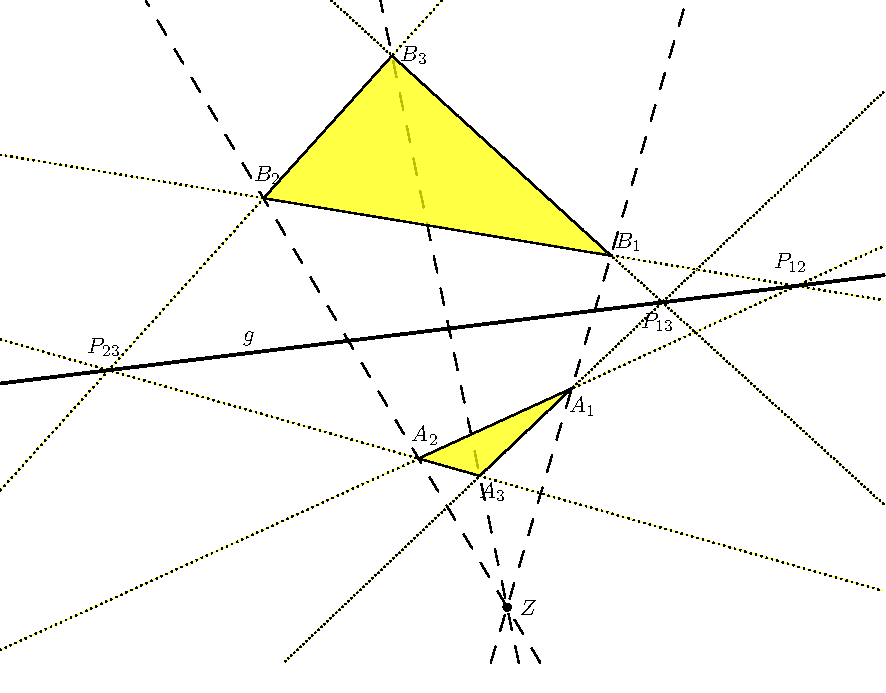
\includegraphics[width=12cm]{img/desargues}
\end{figure}

\begin{thm}
 Sei $V$ ein $K$-Vektorraum über einem Schiefkörper $K$ mit $\dim V \ge 3$. Dann ist $\proj(V)$ desarguessch.
\end{thm}

\begin{proof}
 Falls $Z$ mit einer Ecke übereinstimmt ist die Behauptung trivial. Sei also o.B.d.A. $Z \ne A_i$, $Z \ne B_i$, $A_i \ne B_i$ für $i = 1,2,3$. Seien $Z = [v]$, $A_i = [v_i]$. 
 
 Wir können nun $B_i = [v + v_i]$, $i = 1,2,3$ annehmen. Begründung: Wähle $v$ fest und $\tilde{v}_i$ mit $[\tilde{v}_i] = A_i$. Dann sind $B_i = [\lambda_i v + \mu_i \tilde{v}_i]$ für gewisse $\lambda_i, \mu_i \in K$. Es gilt $\lambda_i \ne 0$ weil $B_i \ne Z$ und $\mu_i \ne 0$ weil $B_i \ne A_i$. Also gilt 
 \[ B_i = \lambda_i^{-1} [\lambda_i v + \mu_i \tilde{v}_i] = [v + \underbrace{\lambda_i^{-1} \mu_i \tilde{v}_i}_{=: v_i}] = [v + v_i], \]
 $A = [v_i]$ weil $[\tilde{v_i}] = [v_i]$. Damit folgt 
 \[ P_{12} = A_1 A_2 \cap B_1 B_2 = [v_1 , v_2] \cap [v + v_1, v + v_2 ] = [v_1 - v_2], \]
 denn die projektiven Geraden $A_1 A_2$ und $B_1 B_2$ sind nach Voraussetzung verschieden, also
 \[ \dim( [v_1, v_2] \cap [v + v_1, v + v_2 ] ) = 2 + 2 - \dim[v_1, v_2, v] = 1 \]
 und $v_1 - v_2 \in [v_1, v_2] \cap [v + v_1, v + v_2]$, der Punkt $v_1-v_2$ liegt sowohl in der linearen Hülle von $(v_1, v_2)$ als auch in $(v + v_1, v + v_2)$.

 Entsprechend folgen $P_{23} = [v_2 - v_3]$, $P_{13} = [v_1 - v_3]$. Also liegen $P_{12}$, $P_{13}$, $P_{23}$ auf der projektiven Geraden $[v_1 - v_2, v_2 - v_3]$. Damit gilt in $\proj(V)$ der Satz von Desargues.
\end{proof}

\begin{defn*}
 Sei $\proj$ ein projektiver Raum. In $\proj$ \emph{gilt der Satz von Pappos}\footnote{Pappos von Alexandria, ca. 300}, falls für je 7 verschiedene Punkte $Z, A_1, A_2, A_3, B_1, B_2, B_3$ gilt:
 \begin{addmargin}[.5cm]{0cm} 
 Falls $Z, A_1, A_2, A_3$ auf einer Geraden $g$ liegen und $Z, B_1, B_2, B_3$ auf einer Geraden $h \ne g$ liegen, dann sind die Punkte 
 \[ P_{12} := A_1 B_2 \cap A_2 B_1, \quad P_{23} := A_2 B_3 \cap A_3 B_2, \quad P_{13} := A_1 B_3 \cap A_3 B_1 \]
 kollinear.
 \end{addmargin}
\end{defn*}

\begin{figure*}[ht]
 \center
 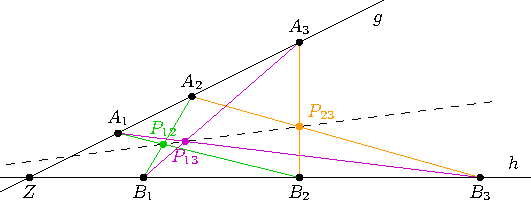
\includegraphics[width=12cm]{img/pappos}
\end{figure*}

\begin{thm}
 Sei $V$ ein $K$-Vektorraum über einem Schiefkörper $K$ und $\dim V \ge 3$. Dann gilt in $\proj(V)$ der Satz von Pappos genau dann, wenn $K$ kommutativ, also ein Körper ist.
\end{thm}

\begin{proof}
 Seien 
 \[ \begin{aligned}
     Z   &:= g \cap h = [u], \\
     A_1 &:= [v] \text{ und o.B.d.A. } A_2 = [u + v] \text{ (ersetze ggf. $v$ durch ein geeignetes $\lambda v$)}, \\
     B_1 &:= [w] \text{ und o.B.d.A. } B_2 = [u + w].
    \end{aligned} \]
 $u, v, w$ sind linear unabhängig, da $g \ne h$. Dann ist $P_{12} = A_1 B_2 \cap A_2 B_1 = [u + v + w]$. 
 
 ``$\Leftarrow$'' Sei $K$ ein Körper. Zu zeigen: $P_{12}, P_{13}, P_{23}$ sind kollinear.
 
 Für $A_3, B_3$ gibt es $r, s \in K$ mit $A_3 = [ru+v]$, $B_3 = [su+w]$. Dann ist 
 \[ P_{13} = A_3 B_1 \cap A_1 B_3 = [ru + v, w] \cap [v, su + w] = [rsu+sv+rw] =: [v_{13}], \]
 denn $s(ru+v) + rw = rsu + sv + rw = sv + r(su + w)$. Dabei gilt $rs = sr$, weil $K$ kommutativ ist.
 \[ P_{23} = A_2 B_3 \cap A_3 B_2 = [u+v, su + w] \cap [ru + v, u+w] \]
 und es gilt
 \[ \begin{aligned}
    (rs-1)u + (s-1)v + (r-1)w 
    &= (s-1) (u+v) + (r-1)(su +w) \\
    &= (s-1)(u+w) + (s-1)(ru+v),
    \end{aligned} \]
 also folgt
 \[ P_{23} = [ (rs-1)u + (s-1)v + (r-1)w ] =: [v_{23}]. \]
 Wir sehen nun $v_{13} - v_{23} = u + v + w \in [u + v + w] = P_{12}$, also sind $P_{12}, P_{13}, P_{23}$ kollinear.
 
 ``$\Rightarrow$'' Gelte der Satz von Pappos. Zu zeigen: $K$ ist ein Körper, also $rs = sr$ für $r,s \in K$.
 
 Seien o.B.d.A.\footnote{Wir schließen 0 und 1 aus, da sie mit allen Elementen von $K$ kommutieren.} $r,s \in K \setminus \{ 0, 1 \}$, $A_3 := [ru+v]$, $B_3 := [su+v]$. Dann gibt es $x,y \in V$ mit $[x+y] = [u + v + w]$.
 
 Seien $P_{13} = [x]$, $P_{23} = [y]$, dann gibt es wegen des Satzes von Pappos $t_1, \ldots, t_8 \in K$, so dass
 \begin{align*}
    x &=   &   t_1 v + t_2 (su+w) &= t_3 w + t_4 (ru+v) \tag{1} \\
    y &=   &   t_5 (u+v) + t_6 (su+w) &= t_7 (u+w) + t_8 (ru+v) \tag{2} \\
  x+y &=   &   u+v+w &= t_1 v + t_2 (su+w) + t_5 (u+v) + t_6 (su+w) \tag{3}
 \end{align*}
 Weil $u,v,w$ linear unabhängig sind, folgt aus (3)
 \[ \left. \begin{aligned}
    w: \quad 1 &= t_2 + t_6 \\
    u: \quad 1 &= (t_2+t_6) s + t_5 = s + t_5 \\
    v: \quad 1 &= t_1 + t_5
    \end{aligned}
    \quad \right\} \Rightarrow 
    \begin{aligned}
     t_1 &= s, \\
     t_2 &= 1 - t_6, \\
     t_5 &= 1 - s. 
    \end{aligned} \]
 Zusammen mit (1) folgt
 \[ v: \quad t_4 = t_1 = s, \qquad u: \quad t_2 s = t_4 r, \qquad w: \quad t_2 = t_3. \]
 Mit $t_2 = 1 - t_6$ aus (3) gilt also
 \[ (1-t_6)s = t_2 s = t_4 r = sr \qRq t_6 s = s - sr \qRq t_6 = 1 - srs^{-1}. \tag{$\circ$} \]
 Zusammen mit (2) folgt
 \[ u: \quad t_5 + t_6s = t_7 + t_8 r, \qquad v: \quad t_8 = t_5, \qquad w: \quad t_7 = t_6. \]
 Nun setzen wir ($\circ$) und $t_5 = 1-s$ ein:
 \begin{align*}
     t_5 + t_6 s = t_6 + t_5 r \quad
     &\Rightarrow & (1-s) + (s-sr) &= (1 - srs^{-1}) + (1-s)r \\
     &\Rightarrow & -srs^{-1} + r &= 0 \\
     &\Rightarrow & srs^{-1} &= r \\
     &\Rightarrow & rs &= sr. \qedhere 
 \end{align*}
\end{proof}

\begin{bem}
 Aus dem Beweis des Satzes folgt in $\proj(V)$ ($V$ ist ein $K$-Vektorraum mit $\dim V \ge 3$): $K$ kommutativ $\Leftrightarrow$ Es existieren paarweise verschiedene $Z, A_1, A_2, B_1, B_2 \in \proj(V)$ mit $Z = A_1 A_2 \cap B_1 B_2$. Für alle $A_3$ auf $A_1 A_2$ mit $A_3 \ne A_1, A_2$ und $B_3$ auf $B_1 B_2$ mit $B_3 \ne B_1, B_2$ gilt: $P_{ij} = A_i B_j \cap A_j B_i$, $i \ne j$ sind kollinear.
 
 Das heißt im Satz von Pappos kann man $Z, A_1, A_2, B_1, B_2$ fest wählen.
\end{bem}

\begin{deno*}
 Der Vektor $x \ne 0$ aus $K^n$ heißt \emph{homogene Koordinaten} von $[x] \in \proj(V)$. Falls $x \in K^n$ mit $x_n \ne 0$, dann ist
 \[ \left[ \begin{pmatrix} x_1 \\ \vdots \\ x_{n-1} \\ x_n \end{pmatrix} \right] =
    \left[ \begin{pmatrix} x_n^{-1} x_1 \\ \vdots \\ x_n^{-1} x_{n-1} \\ 1 \end{pmatrix} \right]. \]
\end{deno*}

Für $V = \real^n$ ist
\[ [x] = \left[ \frac{x}{\|x\|} \right] = \left[ \frac{-x}{\|x\|} \right]. \]
Der projektive Raum $\proj(\real^n)$ kann daher mit der $S^{n-1} \subseteq \real^n$ nach Identifikation von Antipodenpaaren identifiziert werden.
 
$S^{n-1}$ ist die Einheitssphäre. $x \in S^{n-1}$ heißt $x \in \real^n$, $\| x \| = 1$. Wir betrachten also statt Geraden die äquivalenten (gegenüberliegenden) Punkte der Einheitssphäre $S^{n-1}_\pm$, das heißt $x \sim x' \Leftrightarrow x = x'$ oder $x = -x'$.

\subsection*{Dualität für projektive Ebenen}
\begin{thm}
 Sei $\proj = (P,G,I)$ eine projektive Ebene. Dann ist auch $\proj^* := (G,P,I^{-1})$ mit $I^{-1} := \{ (g,p) : (p,g) \in I \}$ eine projektive Ebene.
\end{thm}

$\proj^*$ ist die zu $\proj$ \emph{duale Ebene}. Offensichtlich gilt $\proj^{**} = \proj$.

\begin{proof}
 Zu zeigen: $\proj^*$ erfüllt die Axiome der projektiven Ebene A1), A2'), A3) und A4) (siehe S. \pageref{def:proj}).
 \begin{enumerate}[\hspace{.5cm}A2)]
  \item[A1)] Durch je zwei (verschiedene) Punkte $p_1$, $p_2$ geht genau eine Gerade.
  \item[A2')] Je zwei Geraden schneiden sich.
  \item[A3)] Auf jeder Geraden liegen mindestens drei Punkte.
  \item[A4)] Es gibt mindestens zwei Geraden.
 \end{enumerate}
 
 Die zu einer Aussage über $(P,G,I)$ duale Aussage ist die entsprechende Aussage für $(G,P,I^{-1})$\footnotemark.
 \footnotetext{Vertausche die Rollen von Punkten und Geraden und $I$ mit $I^{-1}$. Begriffe werden analog dualisiert, zum Beispiel die Gerade $P_1 P_2$ entspricht dem Punkt $g_1 \cap g_2$. Kollineare Punkte entsprechen kopunktalen Geraden.}
 
 Aus A1) und A2') folgt die Aussage:
 \begin{enumerate}[\hspace{.5cm}A2)]
  \item [$\widetilde{\text{A2}}$')] Je zwei Geraden schneiden sich in genau einem Punkt.
 \end{enumerate}

 Für die ersten beiden dualen Axiome folgt:
 \begin{enumerate}[\hspace{.5cm}{A}1 {dual})]
  \item[A1 dual)] ist offenbar dieselbe Aussage wie $\widetilde{\text{A2}}$').
  \item[A2' dual)] ist dieselbe Aussage wie A1).
 \end{enumerate}

 Die zu A3) und A4) dualen Aussagen sind
 \begin{enumerate}[\hspace{.5cm}{A}1 {dual})]
  \item[A3 dual)] Durch jeden Punkt gehen mindestens drei Geraden.
  \item[A4 dual)] Es gibt mindestens zwei Punkte.
 \end{enumerate}
 Aus A3) und A4) folgt offenbar A4 dual). 
 
 Zu zeigen: In $\proj$ gilt A3 dual). Sei $P$ ein Punkt. Dann gibt es nach A1) eine Gerade $g$ durch $P$.  Auf dieser liegen nach A3) mindestens zwei weitere Punkte $P_1$ und $P_2$. Nach A4) gibt es mindestens eine weitere Gerade $h$ und nach A2') schneiden sich $g$ und $h$ in einem Punkt $X$. Auf $h$ gibt es nach A3) zwei Punkte $Q_1, Q_2 \ne X$. Die Geraden $PQ_1, PQ_2$ und $PP_1$ sind paarweise verschieden. Damit gibt es mindestens drei Geraden durch $P$.
\end{proof}

\textbf{Dualitätsprinzip.} Wenn eine Aussage für alle projektiven Ebenen gilt, dann gilt auch die duale Aussage für alle projektiven Ebenen\footnote{Vertausche zum Beweis einfach $\proj$ mit $\proj^*$.}.

\begin{exmp*}
 Dualisiere die Aussage ``$\proj = (P,G,I)$ ist desarguessch.'' Beweise: Wenn $\proj$ desarguessch ist, dann ist es auch $\proj^*$.
 
 \begin{addmargin}[.5cm]{0cm} 
 \textbf{Aussage von Desargues.} Für alle $A_1, A_2, A_3, B_1, B_2, B_3 \in P$ mit $A_i \ne B_i$, sodass $A_1, A_2, A_3$ nicht kollinear sind und $B_1, B_2, B_3$ nicht kollinear sind, gilt: Falls $Z$ der Schnittpunkt von $A_1 B_1$, $A_2 B_2$ und $A_3 B_3$ ist, dann sind 
 \begin{align*}
  P_{12} &:= A_1 A_2 \cap B_1 B_2, \\
  P_{23} &:= A_2 A_3 \cap B_1 B_2, \\
  P_{13} &:= A_3 A_1 \cap B_3 B_1 
 \end{align*}
 kollinear.
 
 \textbf{Duale Aussage.} Für alle $g_1, g_2, g_3, h_1, h_2, h_3 \in G$ mit $g_i \ne h_i$, sodass $g_1, g_2, g_3$ nicht kopunktal\footnote{Das heißt, dass die drei Geraden sich nicht in \emph{einem} Punkt schneiden, sondern ein Dreieck bilden.} und $h_1, h_2, h_3$ nicht kopunktal sind, gilt: Falls $f$ eine Gerade durch $g_1 \cap h_1$, $g_2 \cap h_2$, $g_3 \cap h_3$ ist, dann sind
 \begin{align*}
  l_{12} &:= (g_1 \cap g_2)(h_1 \cap h_2), \\
  l_{23} &:= (g_2 \cap g_3)(h_2 \cap h_3), \\
  l_{31} &:= (g_3 \cap g_1)(h_3 \cap h_1 )
 \end{align*}
 kopunktal.
 \end{addmargin}
\end{exmp*}

\begin{thm}
 Eine projektive Ebene $\proj$ ist desarguessch $\Leftrightarrow$ $\proj^*$ ist desarguessch.
\end{thm}

\subsection*{Endliche projektive Ebenen}
\begin{defn*}
 Ein projektiver Raum $\proj = (P,G,I)$ heißt \emph{endlich}, falls $P$ endlich ist.
\end{defn*}

\begin{deno*}
 Sei $g \in G$, dann bezeichne $(g) := \{ p \in P : (p,g) \in I \}$ die Menge der Punkte auf der Geraden $g$.
\end{deno*}


\end{document}